\subsection{Inbound Latency}
\label{s:eval_inbound}
\iffalse We prototyped the proxy described in \S\ref{s:inbound} on a commodity host (Intel quad core CPU at 2.66Ghz and 8GB RAM). 
We evaluated it using the same setup as described in \S\ref{s:measure_inbound}. 
We found that the proxy almost completely eliminates the inbound delay: 
the delay is under 0.199ms (0.02ms) for a flow arrival rate of 200/s (2000/s); the 99th percentile delay is as small as 0.476ms (3.5ms), which is mainly due to the proxy's software overhead.  
 Since the proxy is physically decoupled from the switch, there is no impact of the switch's \flowmod\ or \packetout\ operations on the proxy's \packetin\ operations. 
In contrast, without the proxy, the mean and 99th percentile delays are 8ms and 192ms respectively, with a flow arrival rate of 200/s. 
These improvements are significant, especially for latency sensitive applications such as VoIP calls in cellular networks. \fi


\begin{figure}[!tb]
\centering
%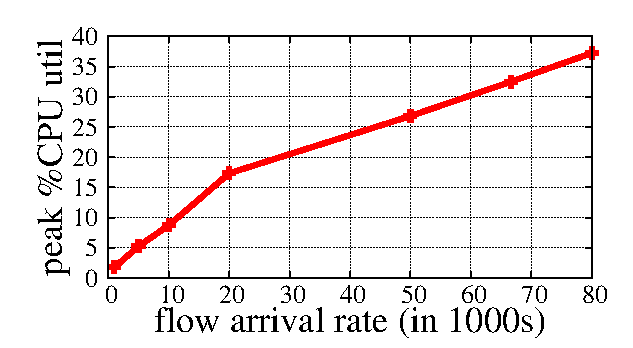
\epsfig{file=./figs/proxyCPU.eps,width=0.35\textwidth}
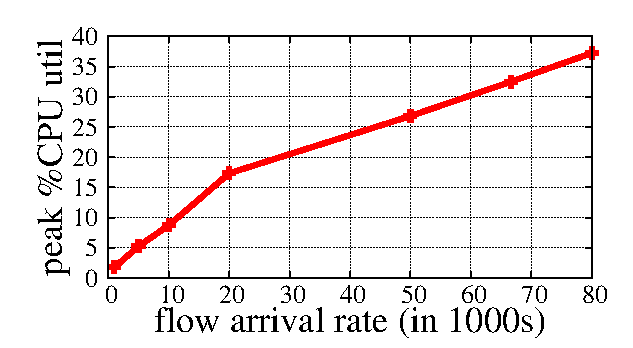
\includegraphics[width=50mm,scale=0.5]{./figs/proxyCPU.eps}
\vspace{0.1em}
\compactcaption{ Peak \%CPU utilization for different \packetin generation rate }\label{peakCPU}
\end{figure}

We prototyped the proxy described in \secref{s:inbound} on a commodity host
(Intel quad-core 2.66GHz CPU, 8GB RAM). We measured the inbound latency
using the same setup as described in \secref{s:measure_inbound}; the only
difference is that the switch now forwards packets at line rate to the proxy,
which generates \packetin messages. At a flow arrival rate of 200/s, we
recorded an average inbound latency of 0.199ms and a 99th percentile latency
of 0.476ms. Even at a much higher flow rate of 2000/s, we recorded values of
0.146ms and 3.56ms for average and 99th percentile inbound latencies
respectively.  Compared with the status quo (average=8ms, 99th percentile=192ms for 200flows/sec) this improvement is substantial, 
especially for latency sensitive applications like VoIP calls in cellular networks. We also note that other operations like \flowmod on the switch do not impact inbound latency as the proxy is physically decoupled from it.

Along with the significant reduction in inbound latency, the solution also
needs to scale to be practically viable. \figref{peakCPU} shows that the peak \%cpu utilization of the proxy at different \packetin generation rates only increases linearly. Furthermore, our prototype is capable of generating 
80,000 \packetin messages per second.
\iffalse\footnote{We can further improve this number using techniques such as Direct NIC Access for packet capture and release.}\fi 
This enables a considerably high number of switches to use a single proxy,
making it a scalable, cost-effective, and efficient immediate solution.

% on average across various rates of incoming traffic. 

% We set the flow table of the switch to be empty so the openflow agent on the switch generates 
% the \packetin messages to the controller. We injected flows at the speed of 500/s, 1000/s and 2000/s and 
% time tamp when the packet is leaving the NIC of the host and when the \packetin messages are received by the openflow controller. 
% For each flow injection rate, we keep the experiments for 30 seconds. The average inbound delays for new flow arrival rate 500/s, 
% 1000/s and 2000/s are 0.0163, 0.0164 and 0.0189 ms respectively. 
% The 99.99\% percentile inbound delays for new flow arrival rate 500/s, 1000/s and 2000/s are 0.092, 1.938 and 3.489 ms, respectively.

